\documentclass[letterpaper,10pt,titlepage,fleqn]{article}

%example of setting the fleqn parameter to the article class -- the below sets the offset from flush left (fl)
\setlength{\mathindent}{1cm}

\usepackage{graphicx}                                        
\usepackage{amssymb}                                         
\usepackage{amsmath}                                         
\usepackage{amsthm} 
\usepackage{esint}
\usepackage{nopageno}
\usepackage{booktabs}                            
\usepackage{alltt}                                           
\usepackage{float}
\usepackage{color}
\usepackage{fancyhdr}
\usepackage{url}
\usepackage{balance}
\usepackage[TABBOTCAP, tight]{subfigure}
\usepackage{enumitem}
\usepackage{pstricks, pst-node}
%the following sets the geometry of the page
\usepackage{geometry}
\geometry{textheight=9in, textwidth=6.5in}
\pagestyle{fancy}
% random comment
\newcommand{\cred}[1]{{\color{red}#1}}
\newcommand{\cblue}[1]{{\color{blue}#1}}
\usepackage{hyperref}
\usepackage{textcomp}
\usepackage{listings}
\def\name{Best CS325 Group}
%% The following metadata will show up in the PDF properties
\hypersetup{
  colorlinks = true,
  urlcolor = black,
  pdfauthor = {\name},
  pdfkeywords = {cs311 ``operating systems'' files filesystem I/O},
  pdftitle = {Pertinent Information},
  pdfsubject = {Virtual Reality Lab},
  pdfpagemode = UseNone
}

\parindent = 0.0 in
\parskip = 0.2 in
\fboxsep=5mm%padding thickness
\fboxrule=4pt%border thickness

\begin{document}
\lstset{language=Python} 

\title{Programming Assignment \#2 - CS325}

\author{
	Joshua Villwock \and
	Jaron Thatcher \and
	Ryan Phillips
}

\date{February 16, 2014}
\maketitle
%to remove page numbers, set the page style to empty







\section*{Introduction}
\hrule

In this writeup, we will both assess time complexity and prove three algorithms designed to solve the Maximum Subarray problem. 

"In computer science, the maximum subarray problem is the task of finding the contiguous subarray within a one-dimensional array of numbers (containing at least one positive number) which has the largest sum. For example, for the sequence of values −2, 1, −3, 4, −1, 2, 1, −5, 4; the contiguous subarray with the largest sum is 4, −1, 2, 1, with sum 6."










\section*{Pseudocode}
\hrule
\begin{centering}

    \textbf{Brute Force:}
    \end{centering}
    \begin{lstlisting}%brute force pseudocode goes here
    \end{lstlisting}

    \begin{centering}
    \textbf{Divide and Conquer:}
    \end{centering}
    \begin{lstlisting}%divide and conquer pseudocode goes here
    \end{lstlisting}

    \begin{centering}
    \textbf{Dynamic Programming:}
    \end{centering}
    \begin{lstlisting}%dynamic programming pseudocode goes here
    \end{lstlisting}











    \section*{Correctness Proofs}
    \hrule

    \begin{centering}
    \textbf{Divide and Conquer:}
    \end{centering}

    %divide and conquer proof goes here

    \begin{centering}
    \textbf{Dynamic Programming:}
    \end{centering}

    %dynamic programming proof goes here







\section*{Asymptotic Analysis of Run Time}
\hrule
\begin{centering}
\textbf{Brute Force:}
\end{centering}

\begin{lstlisting}%brute force asymptotic runtime goes here

\end{lstlisting}

\begin{centering}
\textbf{Divide and Conquer:}
\end{centering}

\begin{lstlisting}%divide and conquer asymptotic runtime here

\end{lstlisting}

\begin{centering}
\textbf{Dynamic Programming:}
\end{centering}

\begin{lstlisting}%dynamic programming asymptotic runtime here

\end{lstlisting}



\section*{Extrapolation and Interpretation}
\hrule

\begin{centering}
\textbf{Slope of lines in log-log plot:}
\end{centering}

The equation for the best fit line on the log-log plot (calculated using numpy.polyfit()) has the following form:

f(n) = e\textsuperscript{y-intercept} * n\textsuperscript{slope}

Brute Force:
\begin{itemize}
\item slope: 2.05692581355
\item y-intercept: -17.5588327907
\end{itemize}

Naive Divide \& Conquer:
\begin{itemize}
\item slope: 2.03626014268
\item y-intercept: -17.3982172216
\end{itemize}

Merge \& Count:
\begin{itemize}
\item slope: 1.10025742067
\item y-intercept: -13.1947528938
\end{itemize}

\begin{centering}
\textbf{Largest input item solvable in an hour:}
\end{centering}





\begin{centering}
\textbf{Discrepancy between actual and asymptotic:}
\end{centering}

The slopes of the first two best fit lines on the log-log graph are very close to 2, and the third is just over 1.1. This matches up with what is expected - i.e. there is no real discrepency to report.

\newpage

\section*{Empirical Analysis of Run Time}
\hrule
\textbf{Linear Plot:}
\vskip 0.04in
\begin{center}
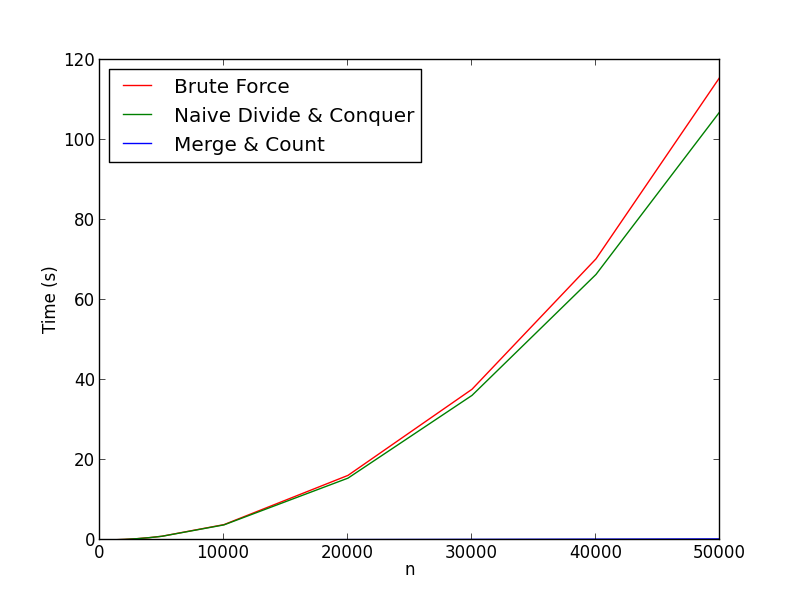
\includegraphics[width=4.5in]{input_time.png}
\end{center}
\textbf{Log-log Plot:}
\vskip 0.04in
\begin{center}
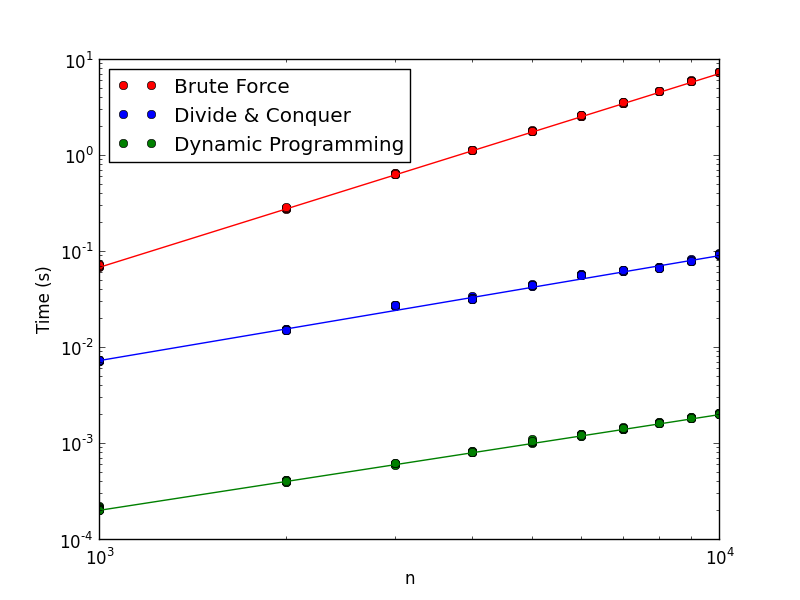
\includegraphics[width=4.5in]{loglog.png}
\end{center}
\end{document}
